 %!TEX root = coexistence_paper.tex



\section{Handling Coexistence In LoRa}\label{sec:coexistence}
  


\subsection{Performance of LoRa under Co-existence}
%To Do.. Add motivational results for LoRaWAN%


\edit{In massive crowds of coexisting networks, the interference pattern can be hard to detect for an LPWAN device like LoRa. Hence, a TDMA (time division multiple access) or traditional CSMA/CA based approach will simply fail.}

%To Do Explain why CSMA/CA and TDMA will not work in detail
 

\subsection{A learning-based approach to co-existence handling}

As the wireless environment is largely unknown due to the coexistence of a massive number of unknown devices/networks,  a {\slshape learning} based approach becomes more effective to make actions (e.g, transmit, sleep, backoff) according to the environmental conditions. However, a learning process usually can be time and computation extensive while the nodes are power-constrained and battery-operated. Hence, we propose to adopt a lightweight machine learning approach. Specifically, as the SNOW nodes may have no knowledge of the coexisting networks, we will adopt  {\bf\slshape Reinforcement Learning (RL)} that enables an {\slshape agent} (e.g., a node) to learn by interacting with its environment~\cite{RLBook}. As shown in Fig.~\ref{fig:reinforcement}, an agent regularly updates its achieved {\slshape rewards} based on the taken action at a given {\slshape state}.  It will learn to take the best actions that maximize its long-term rewards by using its own experience. This would be the {\bf first RL approach} for LPWAN and for handling coexistence for any low-power network. 



 
    \begin{figure}%{r}{4.2cm}
    \centering%\vspace{-0.6in}
    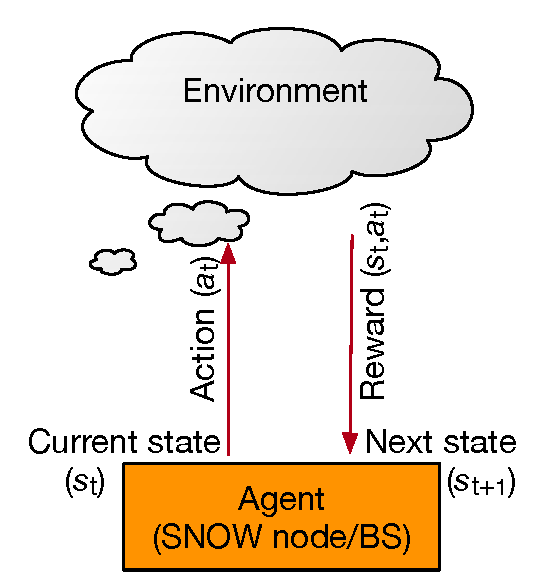
\includegraphics[width=0.22\textwidth]{figs/reinforcement.eps}      
    \vspace{-0.05in}
    \caption{\scriptsize RL visualization}\vspace{-0.1in}
    \label{fig:reinforcement}
 \end{figure}
 
 
\subsection{Rationale for Reinforcement Learning} 
 We adopt {\slshape Q-learning},  a widely-adopted RL technique, which is well-suited for coexistence handling because it is useful in decision making under unknown network conditions. It has {\slshape low memory requirements} and {\slshape low computation}, and learns near-optimal or even {\slshape optimal} solution under certain conditions. Q-learning can be {\slshape efficiently} implemented in a distributed platform like WSN, where each node chooses actions to maximize rewards. It has been efficiently used in cognitive radios~\cite{cognitive1}, and in WSN for routing~\cite{RLRouting1, RLRouting2, RLRouting3, RLRouting4},  QoS provisioning~\cite{QoS1, QoS2}, and resource management \cite{RLSurvey}. It was also used with  RTS/CTS  to learn contention and collision with the nodes in the {\bf same} network  using a {\bf single channel}~\cite{RLMAC}. 
 %SNOW exploits many subcarriers concurrently and does not rely on energy-consuming RTS/CTS frames. 
We aim to adopt RL to handle its coexistence with numerous  unknown and uncoordinated networks. RL has not yet been adopted to handle such coexistence. LPWAN technologies like LoRa has unique features which require a new Q-learning framework. For example, LoRa networks enable multiple concurrent transmissions by dynamically adjusting multiple transmission parameters. Thus, adopting Q-learning for low-power LoRa devices requires a novel Q-learning framework.


\subsection{Challenges for Q-learning in LoRa}
\revise{Like other LPWAN technologies, LoRa devices are extremely low-power and do not possess high computation power. Although Q-learning has low memory and computation requirement compared to other RL approaches, we have to be cautious in designing the Qlearning agent. Specifically, the memory and computation requirement of an Qlearning agent is dependent on the size of the set of actions and agent states. Thus, these parameters need to be chosen carefully to not overwhelm the low-power LoRa devices. }



\section{Design of the LoRa Q-learning Agent}
Every LoRa node will use a Q-learning agent locally for uplink communication. Each Q-learning agent aims to learn the communication pattern of other co-existing networks and take intelligent decisions to increase the network performance. We  consider agent (node) states $\Omega=\{\text{\slshape \small Tx, Rx, Idle, sleep}  \}$, to indicate its state of transmitting, receiving, idle,  and sleeping. Each node will start transmitting on a randomly selected channel from the set of enabled channels in the operating band. After each transmission, the Q-learning agent updates it knowledge about the network through the acknowledgment received from the gateway. 

\subsection{Action Set Formulation}

\noindent{ \bf Is Back-off Advantageous under Coexistence?}

\noindent{In traditional LoRa networks, whenever nodes have data, they transmit immediately . However, that might lead to the transmission being failed. Thus,it might be better to introduce a backoff period before transmissions. Based on the received acknowledgements each Q-learning agent tries to learn the best backoff period which increases the \emph{throughput} and decreases the \emph{energy consumption} under \emph{tolerable} latency.}


\noindent{ \bf Is Channel Hopping Advantageous under Coexistence?}

\noindent{In traditional LoRa, the nodes randomly hop between 64 channels before each transmission. However, our q-learning agent can learn which channel has better probability of making a successful transmission with less number of transmission attempts.}


\noindent{\bf Is Changing SF Advantageous under Coexistence?}

\noindent{LoRa networks usually rely on Adaptive Data Rate(ADR) control from the network server for assigning spreading factor to the nodes. The network server tries to increase the network capacity through th ADR algorithm. However, when there are multiple co-existing networks, the network server of one network can not anticipate the interference caused by other networks. Thus, transmissions on the spreading factor assigned by the network server may not be successful. However, the q-learning agent can learn the best spreading factor which has higher probability of ensuring a successful reception at the gateway.}



%Thus, in our framework ,the network manager initially assigns spreading factors to nodes. Nodes start transmitting using the allocated spreading factors. However, nodes can change their channel and spreading factor after each transmission based on the Q-learning MAC. After each failed transmission,the nodes can choose to transmit in another channel, or transmit using another spreading factor or they can choose to not transmit immediately and back-off. 




 \begin{figure}%[!htpb]%{r}{4.1cm}
    \centering%\hfill
   \label{fig:statediagram_lora}
   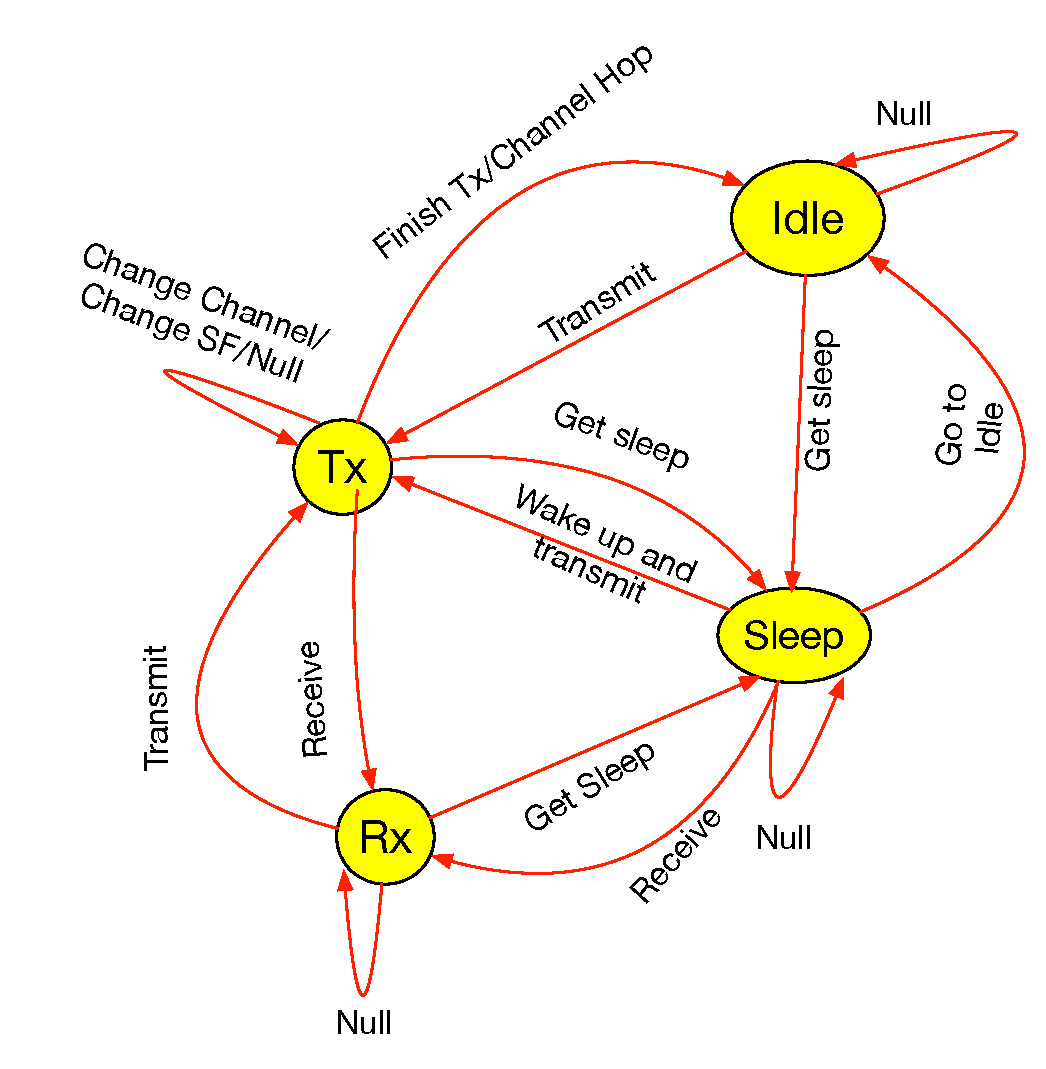
\includegraphics[width=0.4\textwidth]{figs/State_diagram_lora.eps}
      \vspace{-0.15in}
    \caption{\footnotesize Agent state diagram.}%\vspace{-.15in}
 \end{figure}
 
 
Thus, the set of actions is
\vspace{-2mm}
 $$
  \vspace{-2mm}
  \Lambda=\{\text{\slshape \small Transmit, Receive, Backoff, Wake up, Channel hop, Change SF, null}\}$$

\subsection{Reward Function Formulation}
Let $s_t\in \Omega$  be the agent state at time $t$. Its total reward is given by 
 \vspace{-2mm}
 $$
\vspace{-2mm}
 R(s_t, a_t) = r(s_t, a_t) + c(s_t, a_t),$$
where $r(s_t, a_t)$ is the {\slshape immediate reward}  and $c(s_t, a_t)$ is the {\slshape cost} of taking action $a_t\in \Lambda$  at state $s_t$. Considering both energy consumption and throughput, we can assign some numerical values indicating rewards and costs. As an example, we can consider total reward for a successful packet {\slshape transmission} or {\slshape reception} by considering 2 units of immediate reward  and 1 unit of cost. Thus, a failed transmission will incur only a cost of 1 unit. We can also consider 1 unit of cost in {\slshape idle} state (as the radio consumes energy almost similar to Tx/Rx). From $s_t=${\slshape Idle}, important reward functions can be given as follows. 


\revise{
\begin{footnotesize}
$$%\vspace{-1mm}
R(s_t, a_t) =
\begin{cases}
2 - 1 = 1   & \text{if }  s_t= \text{\slshape Idle},     ~a_t= \text{{\slshape Transmit} and ACK received}\\
0 - 1 = -1   & \text{if } s_t= \text{\slshape Idle},     ~a_t= \text{{\slshape Transmit} and ACK not received}\\
2 - 1 = 1   & \text{if } s_t= \text{\slshape Idle},     ~a_t= \text{\slshape Receive}\\
- 1   & \text{if } s_t= \text{\slshape Idle},     ~a_t= \text{\slshape Null}\\
0   & \text{if } s_t= \text{\slshape Idle},     ~a_t= \text{\slshape Get sleep}
\end{cases}
$$\end{footnotesize}
}

\revise{
\begin{footnotesize}
$$%\vspace{-1mm}
R(s_t, a_t) =
\begin{cases}
2 - 1 = 1   & \text{if }  s_t= \text{\slshape Sleep},     ~a_t= \text{{\slshape Transmit} and ACK received}\\
0 - 1 = -1   & \text{if } s_t= \text{\slshape Sleep},     ~a_t= \text{{\slshape Transmit} and ACK not received}\\
2 - 1 = 1   & \text{if } s_t= \text{\slshape Sleep},     ~a_t= \text{\slshape Receive}\\
 0   & \text{if } s_t= \text{\slshape Sleep},     ~a_t= \text{\slshape Null}\\
-1   & \text{if } s_t= \text{\slshape Sleep},     ~a_t= \text{\slshape Wake up}
\end{cases}
$$\end{footnotesize}
}

\revise{
\begin{footnotesize}
$$%\vspace{-1mm}
R(s_t, a_t) =
\begin{cases}
2 - 1 = 1   & \text{if }  s_t= \text{\slshape Tx},     ~a_t= \text{{\slshape Finish Tx} and ACK received}\\
0 - 1 = -1   & \text{if } s_t= \text{\slshape Tx},     ~a_t= \text{{\slshape Finish Tx} and ACK not received}\\
- 1   & \text{if } s_t= \text{\slshape Tx},     ~a_t= \text{{\slshape Backoff}}\\
- 1   & \text{if } s_t= \text{\slshape Tx},     ~a_t= \text{{\slshape Channel hop and remain Idle}}\\
2 - 1 = 1   & \text{if } s_t= \text{\slshape Tx},     ~a_t= \text{{\slshape Channel hop, transmit and ACK received}}\\
- 1 = 1   & \text{if } s_t= \text{\slshape Tx},     ~a_t= \text{{\slshape Channel hop, transmit and ACK not received}}\\
2 - 1 = 1   & \text{if } s_t= \text{\slshape Tx},     ~a_t= \text{{\slshape Change SF, transmit and ACK received}}\\
- 1 = 1   & \text{if } s_t= \text{\slshape Tx},     ~a_t= \text{{\slshape Change SF, transmit and ACK not received}}\\
-1   & \text{if } s_t= \text{\slshape Tx},     ~a_t= \text{\slshape Null}\\
0   & \text{if } s_t= \text{\slshape Tx},     ~a_t= \text{\slshape Get Sleep}
\end{cases}
$$\end{footnotesize}
}
\revise{
\begin{footnotesize}
$$%\vspace{-1mm}
R(s_t, a_t) =
\begin{cases}
2 - 1 = 1   & \text{if }  s_t= \text{\slshape Rx},     ~a_t= \text{{\slshape Finish Rx}}\\
2 - 1 = 1   & \text{if } s_t= \text{\slshape Rx},     ~a_t= \text{{\slshape Transmit} and ACK received}\\
0 - 1 = - 1   & \text{if } s_t= \text{\slshape Rx},     ~a_t= \text{{\slshape Transmit} and ACK not received}\\
- 1   & \text{if } s_t= \text{\slshape Rx},     ~a_t= \text{{\slshape go to idle}}\\
-1   & \text{if } s_t= \text{\slshape Rx},     ~a_t= \text{\slshape Null}\\
0   & \text{if } s_t= \text{\slshape Rx},     ~a_t= \text{\slshape Get Sleep}
\end{cases}
$$\end{footnotesize}}

 
 
\subsection{ Q-Values and Action Selection Approach} 
Let the Q-value associated with action $a_t$ and state $s_t$ be $Q(s_t, a_t)$. It represents the currently expected total future reward and  is initialized to zero. 
Through trial and experience, the agent learns how good some action was. The Q-values of
the actions change through learning and finally represent the absolute value function. After
convergence, taking the actions with the greatest Q-values in each state guarantees taking an 
optimal decision. The new Q-value of pair $\{s_{t+1}, a_t\}$ in state $s_{t+1}$ after taking action $a_t$ in state $s_t$ is computed
as the sum of old Q-value and a correction term as 

$$
Q(s_{t+1}, a_t) = Q(s_t, a_t) + \gamma(R(s_t, a_t) - Q(s_t, a_t)). $$


The learning constant, $\gamma$, prevents the Q-values from changing too
fast and thus oscillating. The nodes take actions  and update the Q-values up to a certain time length.  After completion, a new episode begins, repeating until the Q-values no longer
change. Always taking the actions with maximum
Q-value (greedy policy) may result in finding locally minimal solutions. On the other
hand, selecting always randomly implies ignoring prior experience and
spending too much energy to learn the complete environment. We shall adopt by combining and weigthing both which is a prominent approach in machine learning~\cite{RLBook}. Specifically, we shall use $\epsilon$-{\bf greedy}: with probability $\epsilon$ the agent takes a random action and with
probability $(1 - \epsilon)$ it takes the best available action, which is known to yield quick and high quality solutions~\cite{RLBook}. 
  
 
 
% \revise{With the above idea, we need to complete our Q-learning framework for both the nodes and the BS to govern the SNOW MAC for handling coexistence..........} 
 Note that every node runs as a single-agent whose Q-table size is $O(|\Omega | . |\Lambda|)$, where $|\Omega |$ is the number states and $|\Lambda|$ is the number of actions. Since these numbers are small for a node, the memory needed is feasible for it. The Q-learning procedure stops after $T$ iterations, called the time {\slshape horizon}, having time complexity $O(T)$. An optimal policy can be achieved as the number of iterations goes to infinity. \revise{The framework can be adopted to other LPWANs by revising the actions and rewards.} 




 
       

          